\documentclass[tikz,border=8pt]{standalone}
\usetikzlibrary{arrows.meta,positioning,shapes.geometric}
\begin{document}
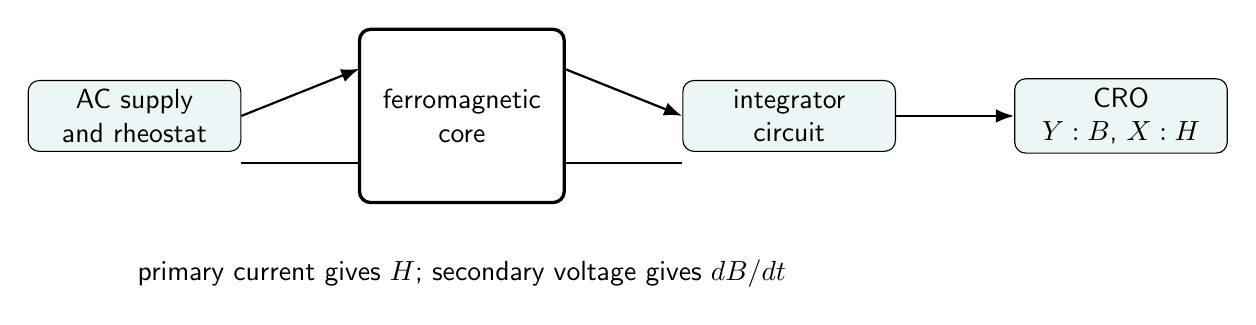
\begin{tikzpicture}[font=\sffamily,>=Latex,box/.style={draw,rounded corners,minimum height=9mm,minimum width=27mm,align=center,fill=teal!7}]
\draw[very thick,rounded corners] (0,0) rectangle (2.6,2.2);
\node[align=center] at (1.3,1.1) {ferromagnetic\\core};
\node[box,left=15mm of {(0,1.1)}] (ac) {AC supply\\and rheostat};
\node[box,right=15mm of {(2.6,1.1)}] (int) {integrator\\circuit};
\node[box,right=15mm of int] (cro) {CRO\\$Y:B$, $X:H$};
\draw[thick,-Latex] (ac.east)--(0,1.7);
\draw[thick] (0,.5)--(ac.east |- 0,.5);
\draw[thick,-Latex] (2.6,1.7)--(int.west);
\draw[thick] (2.6,.5)--(int.west |- 0,.5);
\draw[thick,-Latex] (int.east)--(cro.west);
\node[below=6mm of {(1.3,0)}] {primary current gives $H$; secondary voltage gives $dB/dt$};
\end{tikzpicture}
\end{document}
